\documentclass[aspectratio=169]{beamer}

% ============================================================
% Packages
% ============================================================

\usepackage[spanish,es-nodecimaldot]{babel}
\usepackage[utf8]{inputenc}
\usepackage[T1]{fontenc}
\usepackage{lmodern}
\usepackage{booktabs}
\usepackage{array}
\usepackage{ragged2e}
\usepackage{graphicx}
\usepackage{url}
\usepackage{hyperref}
\usepackage{IEEEtrantools}

% ============================================================
% Professional Beamer visual style
% ============================================================

\usetheme{Boadilla}
\usecolortheme{dolphin}

% Remove navigation symbols
\setbeamertemplate{navigation symbols}{}

% Bibliography style in Beamer
\setbeamertemplate{bibliography item}[text]

% Numbered figures and tables in Beamer
\setbeamertemplate{caption}[numbered]

% ============================================================
% Custom colors
% ============================================================

\definecolor{TecBlue}{RGB}{0,58,112}
\definecolor{TecCyan}{RGB}{0,150,180}
\definecolor{SoftGray}{RGB}{245,247,250}
\definecolor{DarkGray}{RGB}{45,45,45}
\definecolor{LightBlue}{RGB}{232,242,248}

% ============================================================
% Main color configuration
% ============================================================

\setbeamercolor{structure}{fg=TecBlue}
\setbeamercolor{frametitle}{fg=white,bg=TecBlue}
\setbeamercolor{title}{fg=white,bg=TecBlue}
\setbeamercolor{author}{fg=DarkGray}
\setbeamercolor{date}{fg=DarkGray}

% Normal text
\setbeamercolor{normal text}{fg=DarkGray,bg=white}

% Standard blocks
\setbeamercolor{block title}{fg=white,bg=TecBlue}
\setbeamercolor{block body}{fg=DarkGray,bg=SoftGray}

% Alert blocks
\setbeamercolor{alerted text}{fg=TecBlue}
\setbeamercolor{block title alerted}{fg=white,bg=TecCyan}
\setbeamercolor{block body alerted}{fg=DarkGray,bg=LightBlue}

% Example blocks
\setbeamercolor{block title example}{fg=white,bg=TecCyan}
\setbeamercolor{block body example}{fg=DarkGray,bg=SoftGray}

% Itemize bullets
\setbeamercolor{item}{fg=TecCyan}
\setbeamercolor{subitem}{fg=TecBlue}

% Figure captions
\setbeamerfont{caption}{size=\scriptsize}
\setbeamercolor{caption name}{fg=TecBlue}

% Frame title font
\setbeamerfont{frametitle}{series=\bfseries,size=\large}

% Title page font
\setbeamerfont{title}{series=\bfseries,size=\Large}
\setbeamerfont{subtitle}{size=\normalsize}

% ============================================================
% Custom emphasis boxes
% ============================================================

% Important text box without visible title
\newcommand{\importantbox}[1]{
    \begin{beamercolorbox}[
        rounded=true,
        shadow=true,
        wd=\textwidth,
        sep=0.35cm
    ]{block body}
        \justifying
        #1
    \end{beamercolorbox}
}

% Highlighted text box without visible title
\newcommand{\highlightbox}[1]{
    \begin{beamercolorbox}[
        rounded=true,
        shadow=true,
        wd=\textwidth,
        sep=0.35cm
    ]{block body alerted}
        \justifying
        #1
    \end{beamercolorbox}
}

% Compact source/note command
\newcommand{\sourcenote}[1]{
    \vspace{0.1cm}
    \raggedleft
    {\scriptsize #1}
}

% ============================================================
% Dynamic footer section comment
% ============================================================

\newcommand{\rightfootertext}{}
\newcommand{\setrightfooter}[1]{\gdef\rightfootertext{#1}}

\setbeamertemplate{footline}{
  \leavevmode%
  \hbox{%
  \begin{beamercolorbox}[wd=.65\paperwidth,ht=2.5ex,dp=1ex,leftskip=1em]{author in head/foot}%
    \scriptsize Sistema de control ESD
  \end{beamercolorbox}%
  \begin{beamercolorbox}[wd=.35\paperwidth,ht=2.5ex,dp=1ex,rightskip=1em plus1fil]{date in head/foot}%
    \scriptsize \rightfootertext
  \end{beamercolorbox}}%
  \vskip0pt%
}

\setbeamercolor{author in head/foot}{fg=white,bg=TecBlue}
\setbeamercolor{date in head/foot}{fg=white,bg=TecCyan}

% ============================================================
% Presentation metadata
% ============================================================

\title{Diseño y implementación de un sistema inteligente \\ de bajo costo para el control ESD en laboratorios de electrónica}
\author{Randy Zamora Rojas}
\institute{
Anteproyecto de graduación -- Ingeniería Electrónica\\
Instituto Tecnológico de Costa Rica\\[0.2cm]
\textbf{Asesor:} M.Sc. Javier Rivera Alvarado
}
\date{Agosto 2026}

% ============================================================
% Document
% ============================================================

\begin{document}

\bstctlcite{BSTcontrolSpanish}

% ============================================================
% Cover
% ============================================================

\begin{frame}[plain]
  \titlepage
\end{frame}

% ============================================================
% Initial motivation
% ============================================================

\setrightfooter{¿Por qué es importante el control ESD?}

\begin{frame}{Impacto de las descargas electrostáticas}

\importantbox{
Una persona puede generar hasta 35,000 V al caminar \cite{esda_part1},
suficiente para dañar dispositivos electrónicos sensibles. La industria pierde
entre 4\% y 6\% de sus ingresos debido a ESD según Versalogic Corporation
\cite{versalogic_esd_wp}.
}

\begin{figure}
    \centering
    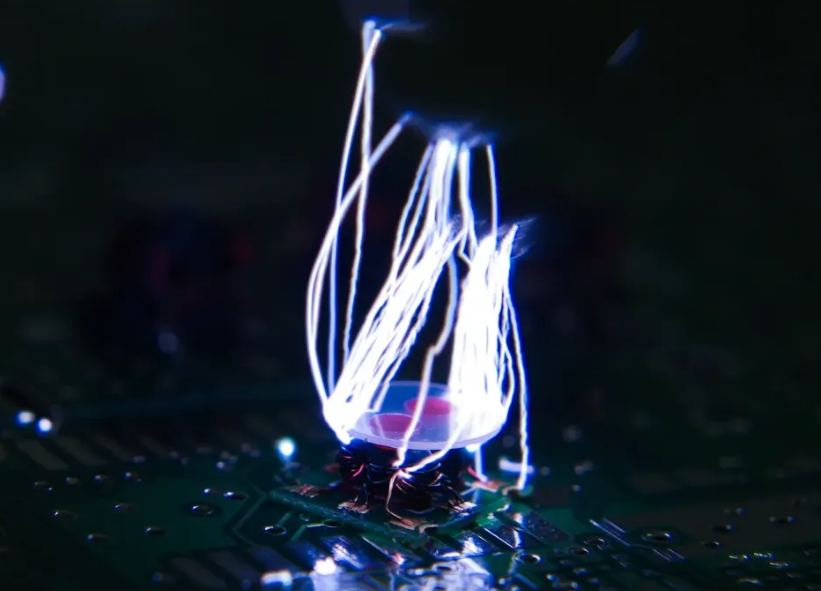
\includegraphics[width=0.38\textwidth]{Figures/F1.png}
    \caption{Descarga electrostática sobre un dispositivo electrónico \cite{istock_esd_sparks}.}
\end{figure}

\end{frame}

% ============================================================
% Agenda
% ============================================================

\setrightfooter{}

\begin{frame}[plain]{Agenda}
    \tableofcontents
\end{frame}

% ============================================================
% Introduction
% ============================================================

\setrightfooter{ ¿Qué es control ESD?}
\section{Introducción}

\begin{frame}{Riesgo ESD durante la manipulación electrónica}

\begin{columns}[c]

    % ---------------- Left image ----------------
    \column{0.48\textwidth}

    \begin{figure}
        \centering
        \includegraphics[width=0.95\linewidth]{Figures/F14.jpg}
        \caption{\scriptsize Manipulación de componentes electrónicos sin pulsera antiestática \cite{magnific_cpu_repair}.}
    \end{figure}

    % ---------------- Right image ----------------
    \column{0.48\textwidth}

    \begin{figure}
        \centering
        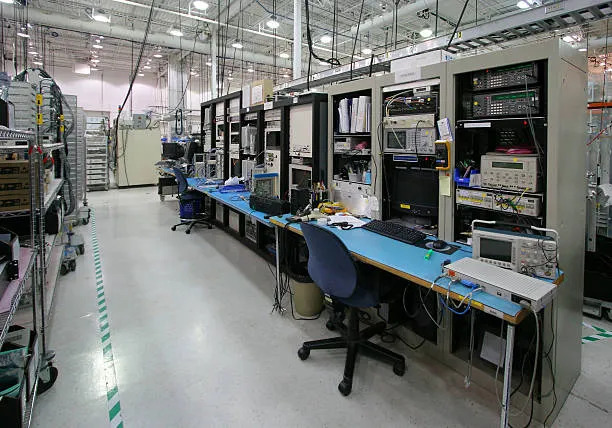
\includegraphics[width=0.95\linewidth]{Figures/IndustrialLab.jpg}
        \caption{\scriptsize Estación de trabajo en ambiente industrial \cite{getty_modern_workstation}.}
    \end{figure}

\end{columns}

\end{frame}

\begin{frame}{Uso de pulsera antiestática}

    \begin{figure}
        \centering
        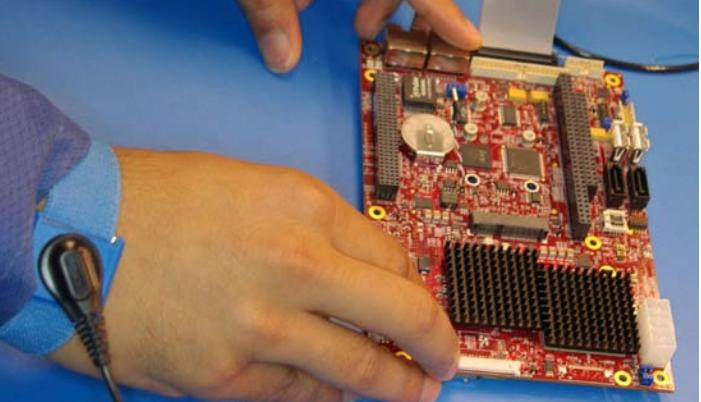
\includegraphics[width=0.6\textwidth]{Figures/F4.jpeg}
        \caption{Uso de pulsera antiestática al manipular componentes electrónicos, fuente: Versalogic Corp \cite{versalogic_esd_wp}.}
    \end{figure}

\end{frame}

\begin{frame}{Sistemas industriales de control ESD}

    \begin{figure}
        \centering
        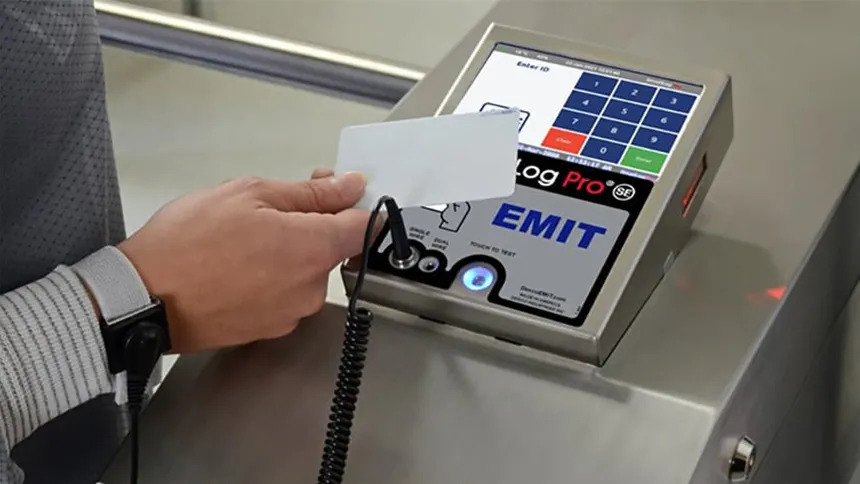
\includegraphics[width=0.7\textwidth]{Figures/F15.jpg}
        \caption{Sistemas de control ESD en industrias \cite{gotopac_esd_access_control}.}
    \end{figure}

\end{frame}

% ============================================================
% Theoretical framework
% ============================================================

\setrightfooter{ ¿Qué es ESD?}
\section{Marco teórico}

\begin{frame}{Generación de carga electrostática y principio físico}

\begin{columns}

    \column{0.72\textwidth}

    \begin{figure}
        \centering
        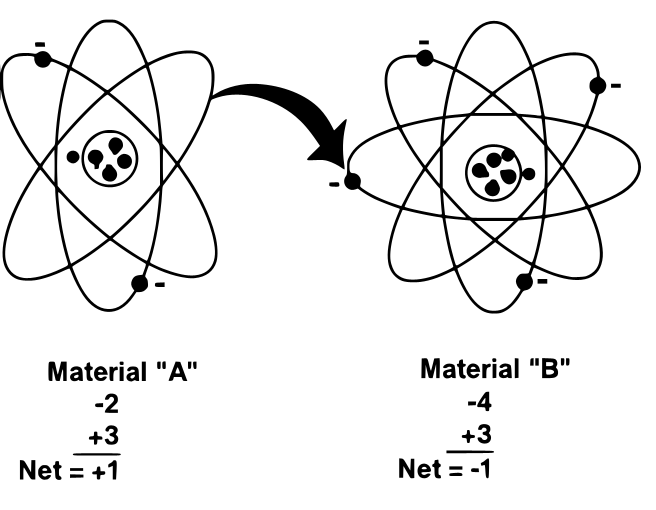
\includegraphics[width=0.65\textwidth]{Figures/F2.png}
        \caption{Generación de carga electrostática por contacto y separación, fuente: ESD Association \cite{esda_part1}.}
    \end{figure}

    \column{0.28\textwidth}

    \begin{block}{Principio físico}
        \centering
        \Large
        \[
            q = C \cdot V
        \]
    \end{block}

    \vspace{0.1cm}

    \centering
    {\scriptsize Fuente: Engineering Electromagnetics, 2019 \cite{hayt2019}}

\end{columns}

\end{frame}

\begin{frame}{Clasificación de materiales según su resistencia eléctrica}

    \begin{figure}
        \centering
        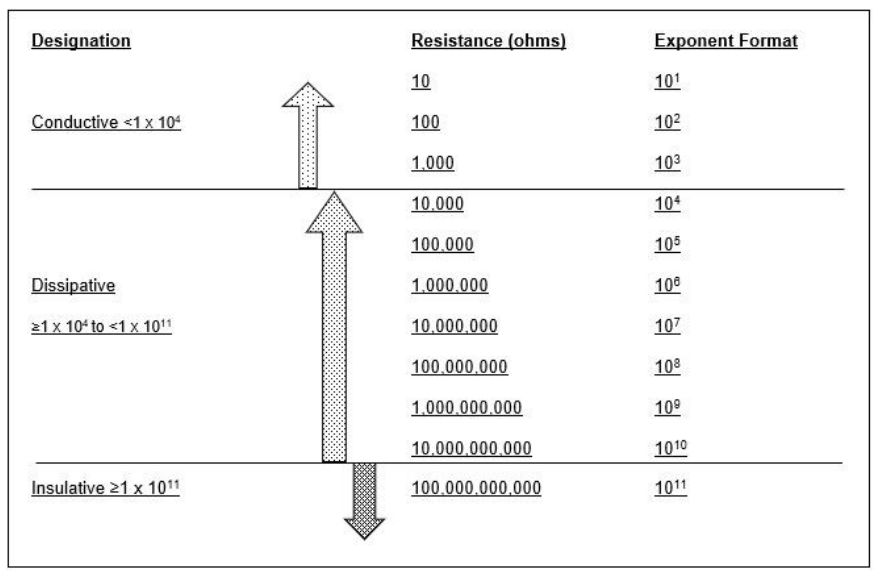
\includegraphics[width=0.6\textwidth]{Figures/F3.png}
        \caption{Clasificación de resistencia eléctrica en materiales, fuente: ESD Association \cite{esda_part1}.}
    \end{figure}

\end{frame}

\begin{frame}{Influencia de la humedad relativa en la generación ESD}

    \begin{table}
    \centering
    \caption{Ejemplos de niveles típicos de voltaje de generación estática, fuente: ESD Association \cite{esda_part1}.}

    \vspace{0.2cm}

    \small
    \renewcommand{\arraystretch}{1.25}

    \begin{tabular}{|p{5.2cm}|c|c|}
        \hline
        \textbf{Medio de generación} & \textbf{10--25\% HR} &
        \textbf{65--90\% HR} \\ \hline
        Caminar sobre alfombra              & 35{,}000 V & 1{,}500 V \\ \hline
        Caminar sobre piso vinílico         & 12{,}000 V & 250 V \\ \hline
        Operario en estación de trabajo     & 6{,}000 V  & 100 V \\ \hline
        Bolsa plástica levantada del banco  & 20{,}000 V & 1{,}200 V \\ \hline
        Silla con espuma de uretano         & 18{,}000 V & 1{,}500 V \\ \hline
    \end{tabular}
    \end{table}

\end{frame}

\begin{frame}{Medición de resistencia cuerpo--tierra}

    \begin{figure}
    \centering
    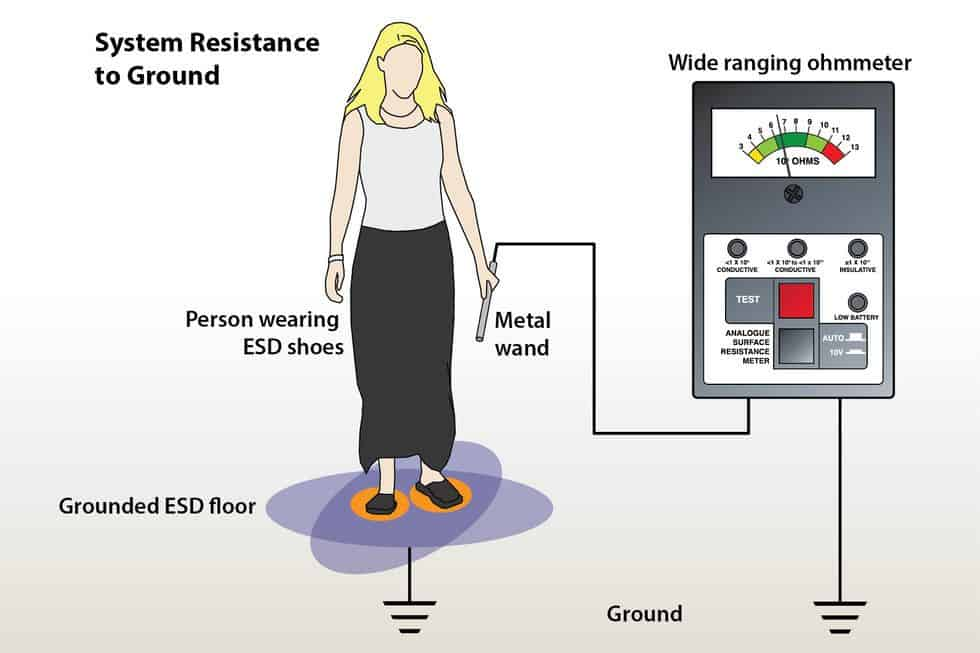
\includegraphics[width=0.6\textwidth]{Figures/TF2_1.jpg}
    \caption{Ilustración de puesta a tierra de una persona, fuente: ESD Association \cite{STM97_ANSI}.}
    \end{figure}

\end{frame}

\begin{frame}{Reto técnico: medición de alta impedancia}

    % ========================================================
    % Top: technical figure
    % ========================================================

    \begin{figure}
        \centering
        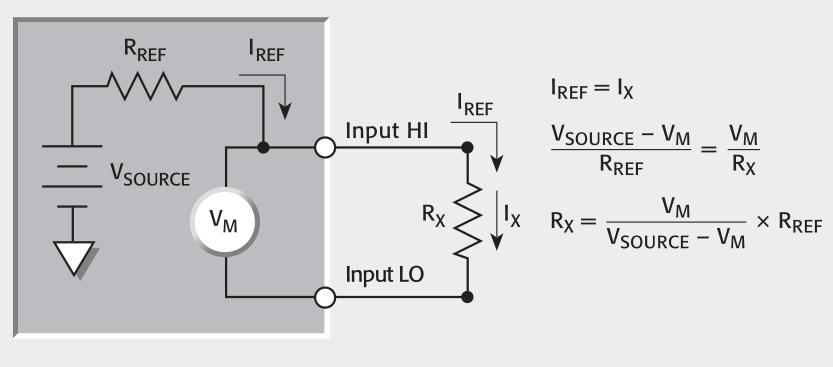
\includegraphics[width=0.62\textwidth]{Figures/TF4_6.png}
        \caption{Ejemplo de corriente de fuga en mediciones de alta impedancia, fuente: Keithley Instruments \cite{keithley_lowlevel}.}
    \end{figure}

    \vspace{-0.15cm}

    % ========================================================
    % Bottom: key idea
    % ========================================================

    \begin{alertblock}{Idea técnica clave}
        En mediciones de alta impedancia, las corrientes de fuga, el aislamiento y el ruido eléctrico pueden afectar el resultado de la medición.
    \end{alertblock}

\end{frame}

% ============================================================
% State of the art
% ============================================================

\setrightfooter{ ¿Qué se ha investigado?}
\section{Estado del arte}

\begin{frame}{Investigación: Monitoreo de puesta a tierra}

\begin{columns}

    % ========================================================
    % Left column: figure
    % ========================================================
    \column{0.45\textwidth}

    \begin{figure}
        \centering
        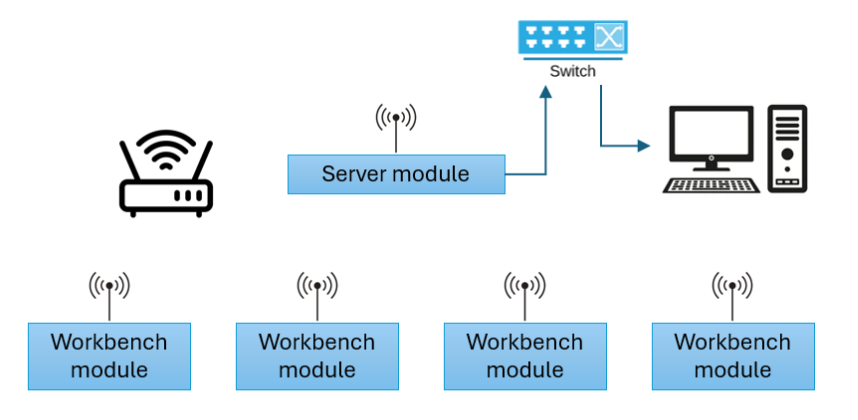
\includegraphics[width=0.82\linewidth]{Figures/SA1_01.png}
        \caption{Monitoreo de resistencia de puesta a tierra \cite{Nagy2025}.}
    \end{figure}

    % ========================================================
    % Right column: relevant information
    % ========================================================
    \column{0.50\textwidth}

    \begin{block}{Aporte principal}
        \small
        Nagy \cite{Nagy2025} propone un sistema IoT para monitorear de forma 
        continua la resistencia de puesta a tierra en estaciones de trabajo 
        ESD.
    \end{block}

    \vspace{0.15cm}

    \begin{block}{Características técnicas}
        \small
        \begin{itemize}
            \item Módulos en estaciones de trabajo.
            \item Servidor central basado en Raspberry Pi.
            \item Comunicación mediante WiFi, MQTT y JSON.
            \item Detección temprana de problemas de conexión a tierra.
        \end{itemize}
    \end{block}


\end{columns}

\end{frame}

\begin{frame}{Investigación: Monitoreo de campos electrostáticos}

\begin{columns}[T]

    % ========================================================
    % Left column: relevant information
    % ========================================================
    \column{0.50\textwidth}

    \begin{block}{Aporte principal}
        \small
        El trabajo de Xu y colaboradores \cite{Xu2023} propone un sistema de monitoreo 
        continuo de ESD para líneas de manufactura, 
        orientado a detectar acumulación de carga electrostática en 
        tarjetas electrónicas ensambladas.
    \end{block}

    \vspace{0.15cm}

    \begin{block}{Características técnicas}
        \small
        \begin{itemize}
            \item Uso de \textit{fieldmeters} sin contacto.
            \item Generación de mapas de calor del campo eléctrico.
            \item Conversión ADC y envío de datos a servidor local.
        \end{itemize}
    \end{block}

    % ========================================================
    % Right column: figure
    % ========================================================
    \column{0.46\textwidth}

    \begin{figure}
        \centering
        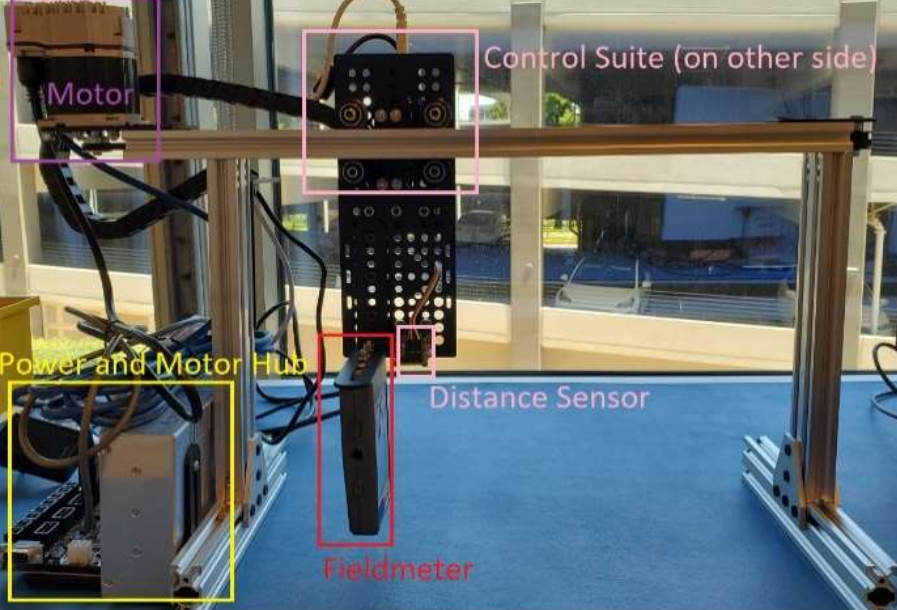
\includegraphics[width=0.82\linewidth]{Figures/SA1_03.png}
        \caption{Monitoreo de campos electrostáticos \cite{Xu2023}.}
    \end{figure}

\end{columns}

\end{frame}

\begin{frame}{Normativas aplicables al control ESD}

\small

\begin{columns}[T]

    % ========================================================
    % Left column: standards
    % ========================================================
    \column{0.43\textwidth}

    \begin{block}{Normativas consideradas}
        \begin{itemize}
            \item \textbf{ANSI/ESD S20.20}
            \item \textbf{IEC 61340-5-1}
            \item \textbf{ANSI/ESD S1.1}
            \item \textbf{ANSI/ESD STM97.1}
            \item \textbf{IEC 60479}
        \end{itemize}
    \end{block}

    \vspace{0.15cm}

    \begin{alertblock}{Parámetros clave}
        \centering
        \textbf{750 k$\Omega$ -- 35 M$\Omega$}\\
        \scriptsize Rango de referencia para verificación de puesta a tierra del personal.
    \end{alertblock}

    % ========================================================
    % Right column: relevance to the project
    % ========================================================
    \column{0.53\textwidth}

    \begin{block}{Importancia para el proyecto}
        \begin{itemize}
            \item \textbf{Programa ESD:} define prácticas de control, verificación y cumplimiento.
            \item \textbf{Pulsera antiestática:} guía la prueba del sistema usuario--pulsera.
            \item \textbf{Calzado/piso ESD:} referencia para resistencia cuerpo--tierra.
            \item \textbf{Seguridad eléctrica:} limita la corriente aplicada al usuario.
            \item \textbf{Trazabilidad:} justifica registrar usuario, fecha, hora y resultado.
        \end{itemize}
    \end{block}

\end{columns}

\vspace{0.1cm}

{\scriptsize Fuente: \cite{ANSI_S2020_Blog},\cite{S1_1_ANSI},\cite{STM97_ANSI},\cite{IEC61340_Preview},\cite{IEC60479}}.

\end{frame}

\setrightfooter{ ¿Qué soluciones existen?}

\begin{frame}{Solución actual en TEM Lab}

\begin{columns}[T]

    \column{0.5\textwidth}

    \begin{figure}
        \centering
        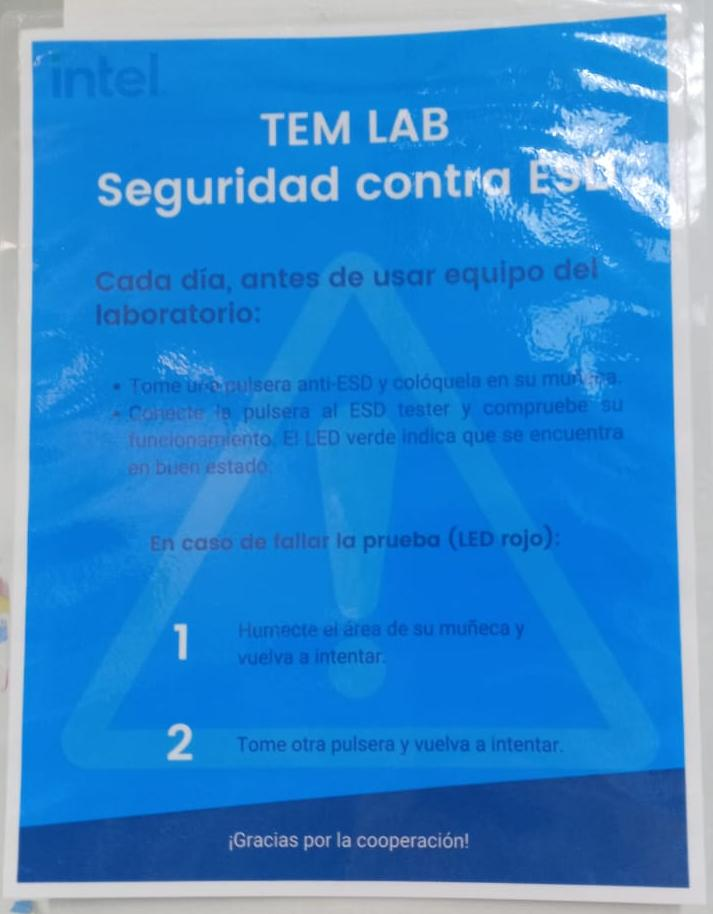
\includegraphics[width=0.6\linewidth]{Figures/F25.jpeg}
        \caption{\scriptsize Indicaciones de seguridad ESD en TEM Lab, fuente: fotografia propia.}
    \end{figure}

    \column{0.5\textwidth}

    \begin{figure}
        \centering
        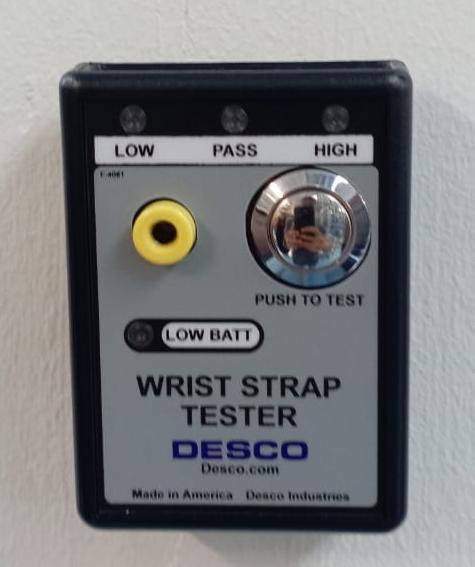
\includegraphics[width=0.6\linewidth]{Figures/F9.jpeg}
        \caption{\scriptsize Tester actual utilizado en TEM Lab, fuente: fotografia propia.}
    \end{figure}

\end{columns}

\end{frame}

\begin{frame}{Sistemas avanzados: ESDMAN}

\begin{columns}[T]

    % ========================================================
    % Left column: product image
    % ========================================================
    \column{0.46\textwidth}

    \begin{figure}
        \centering
        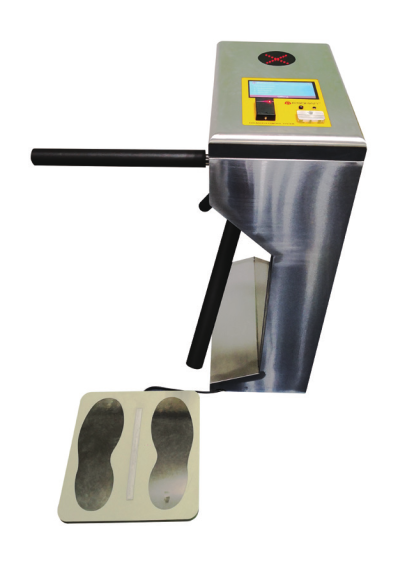
\includegraphics[width=0.6\linewidth]{Figures/F7.png}
        \caption{Sistema ESDMAN \cite{ESDMAN_0016809}.}
    \end{figure}

    \vspace{-0.15cm}

    % ========================================================
    % Right column: main characteristics
    % ========================================================
    \column{0.50\textwidth}

    \begin{block}{Características principales}
        \small
        \begin{itemize}
            \item Identificación de usuario mediante \textbf{RFID}.
            \item Verificación de \textbf{pulsera antiestática}.
            \item Verificación de \textbf{calzado ESD}.
            \item Función de \textbf{control de acceso}.
            \item Interfaz gráfica para operación del sistema.
            \item Generación de reportes y registros de pruebas.
            \item Costo de 2500 USD su versión básica.
            \item Fabricado en China.
        \end{itemize}
    \end{block}

    {\scriptsize \raggedright Fuente: Web oficial de ESDMAN \cite{ESDMAN_0016809}}

\end{columns}

\end{frame}

\begin{frame}{Sistemas avanzados: SmartLog Pro 2}

\begin{columns}

    \column{0.5\textwidth}

   \begin{block}{Características principales}
        \small
        \begin{itemize}
            \item Identificación de usuario mediante \textbf{RFID}.
            \item Verificación de \textbf{pulsera antiestática}.
            \item Verificación de \textbf{calzado ESD}.
            \item Función de \textbf{control de acceso}.
            \item Interfaz gráfica para operación del sistema.
            \item Generación de reportes y registros de pruebas.
            \item Costo de 5643 USD su versión básica.
            \item Fabricado en Estados Unidos
        \end{itemize}
    \end{block}

    {\scriptsize \raggedright Fuente: Web oficial del fabricante \cite{SmartLogPro2}}


    \column{0.5\textwidth}

    \begin{figure}
        \centering
        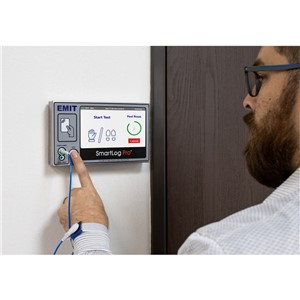
\includegraphics[width=0.8\linewidth]{Figures/SP_22.jpg}
        \caption{EMIT SmartLog Pro 2 \cite{SmartLogPro2}.}
    \end{figure}

\end{columns}

\end{frame}

% ============================================================
% Problem definition
% ============================================================

\setrightfooter{}
\section{Definición del problema}

\begin{frame}{Planteamiento del problema}

    \begin{block}{Situación actual}
        \justifying
        Aunque existen sistemas comerciales para el control ESD en laboratorios de electrónica y
        manufactura de semiconductores, estas soluciones suelen presentar costos elevados y una
        capacidad limitada de personalización. Adicionalmente, no se identifican alternativas de
        bajo costo que integren de manera conjunta la verificación de pulseras antiestáticas, la
        identificación de usuarios, el almacenamiento de registros históricos, la generación de
        reportes y una interfaz gráfica para interactuar con el sistema.
    \end{block}

    \vspace{0.25cm}

    \begin{alertblock}{Necesidad identificada}
        \justifying
        Esta situación evidencia la necesidad de desarrollar una solución accesible y adaptable que
        permita mejorar la trazabilidad de las pruebas ESD en entornos de laboratorio, como el
        laboratorio TEM de Intel Costa Rica, donde se ha identificado una oportunidad de mejora
        en el seguimiento del cumplimiento de los procedimientos ESD.
    \end{alertblock}

\end{frame}

% ============================================================
% Proposed solution
% ============================================================

\setrightfooter{}
\section{Propuesta de solución}

\begin{frame}{¿Cómo proponemos solucionarlo?}

\small

\begin{columns}

    \column{0.45\textwidth}

    \begin{figure}
        \centering
        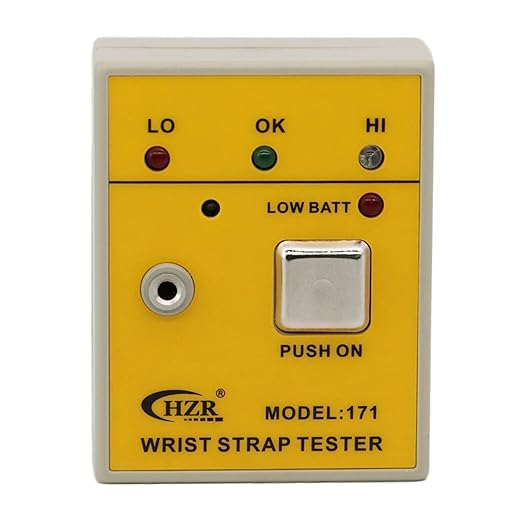
\includegraphics[width=0.75\linewidth]{Figures/F10.jpg}
        \caption{Probador básico de pulsera antiestática HZR171 \cite{HZR171}.}
    \end{figure}

    \column{0.42\textwidth}

    \begin{block}{Características del probador}
        \begin{itemize}
            \item Costo aproximado de 30 USD
            \item Umbrales de prueba de aproximadamente 750 k$\Omega$ y 10 M$\Omega$
            \item Indicación de los estados \textit{LO}, \textit{OK} y \textit{HI}
            \item Alimentación mediante batería de 9 V
        \end{itemize}
    \end{block}

    \vspace{0.15cm}

    \begin{alertblock}{Criterio de selección}
        Permite utilizar una base comercial de prueba y concentrar el desarrollo
        en la identificación, la trazabilidad y la interacción con el usuario.
    \end{alertblock}

\end{columns}

\end{frame}

\begin{frame}{Diagrama de bloques de la solución propuesta}

    \begin{figure}
        \centering
        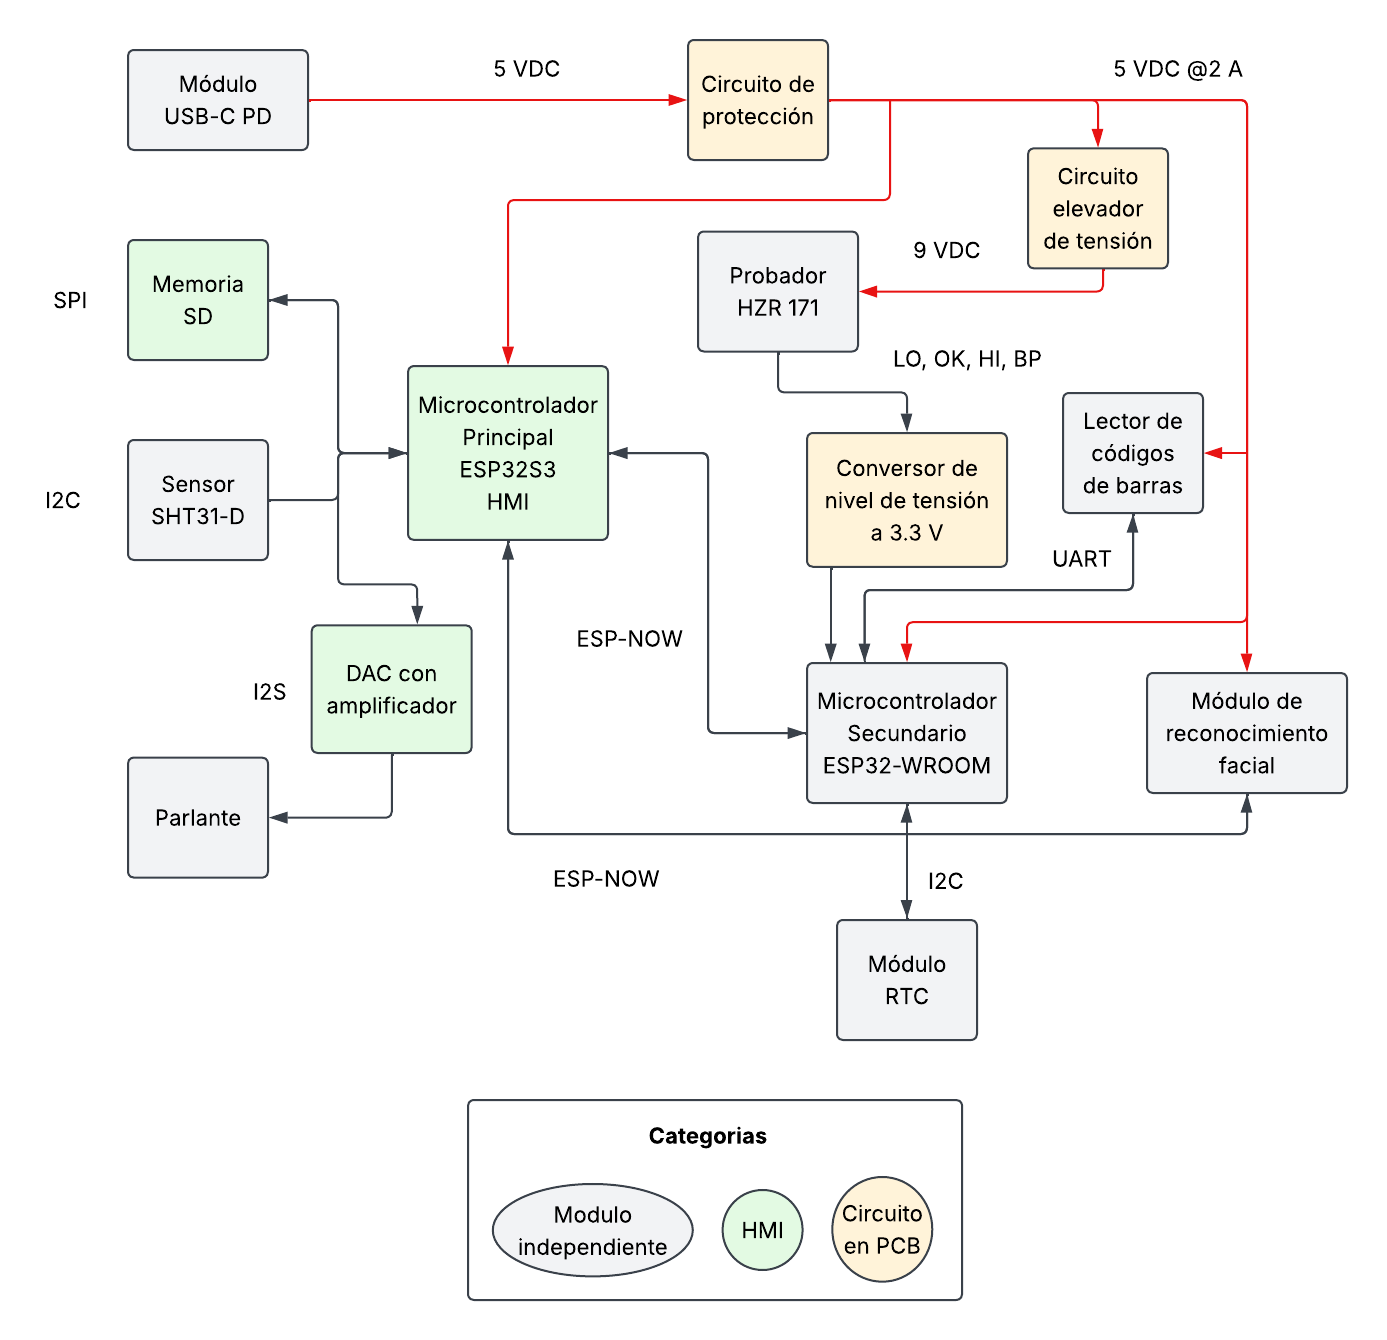
\includegraphics[width=0.98\textwidth,height=0.72\textheight,keepaspectratio]{Figures/SP_16.png}
        \caption{Interconexión de subsistemas del prototipo. Fuente: elaboración propia.}
    \end{figure}

\end{frame}

\begin{frame}{Solución propuesta}

\begin{columns}

    \column{0.45\textwidth}

    \begin{figure}
        \centering
        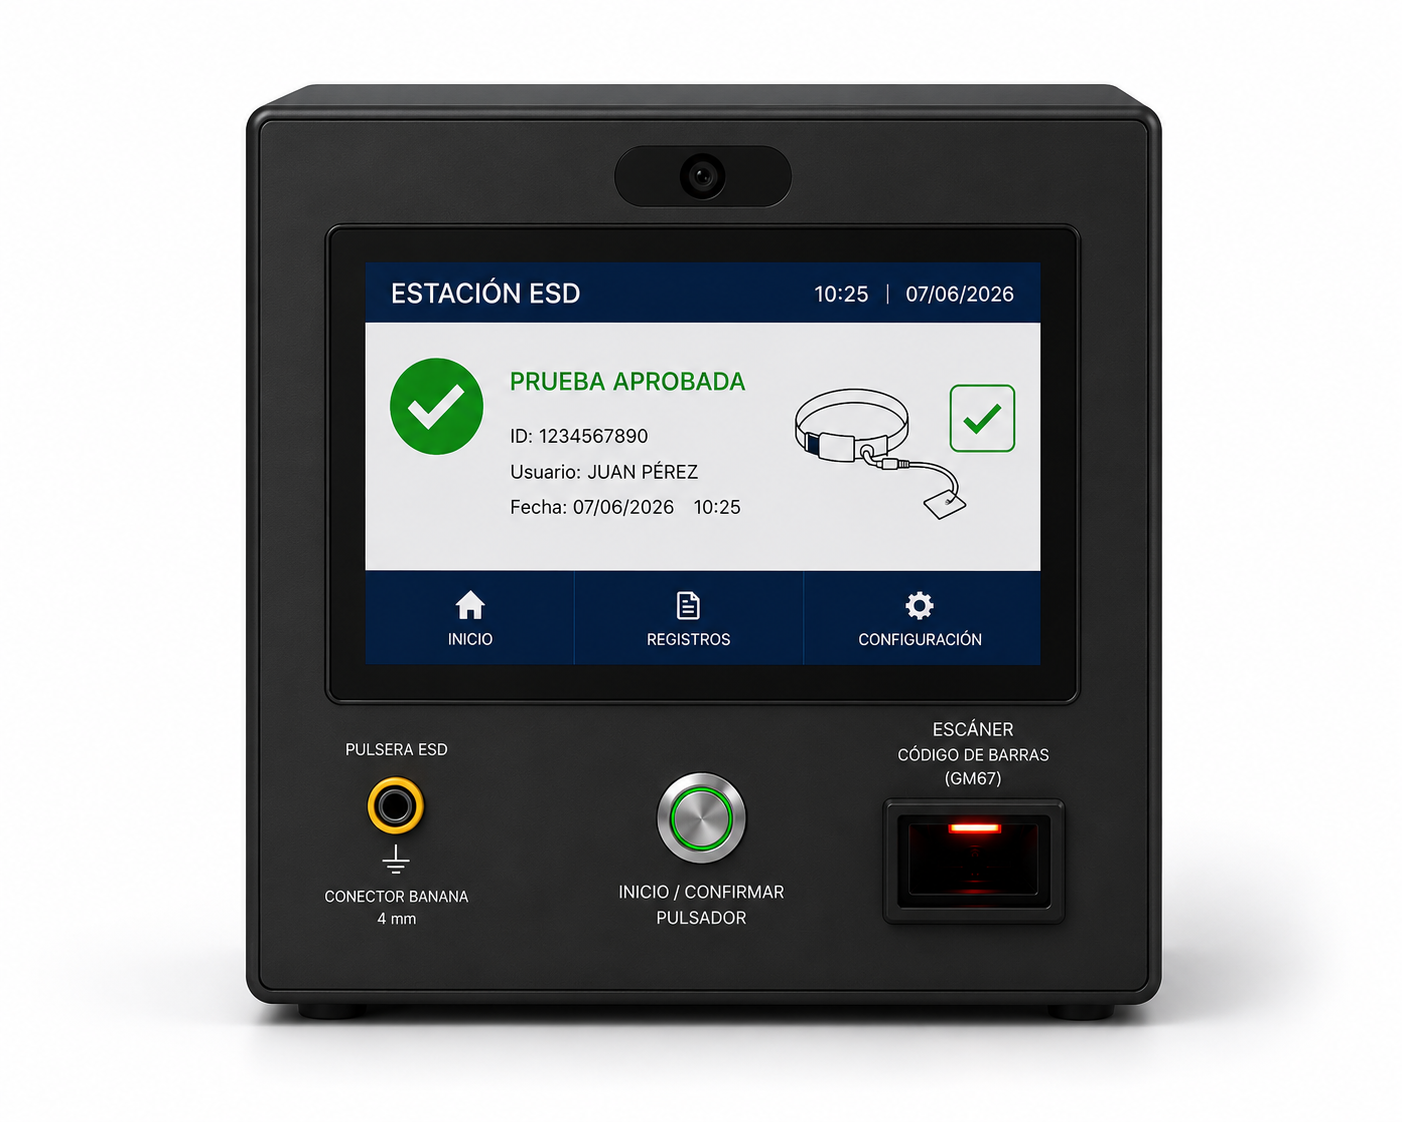
\includegraphics[width=0.9\textwidth]{Figures/SP_20.png}
        \caption{Ilustración del sistema ESD propuesto. Fuente: elaboración propia.}
    \end{figure}

    \column{0.42\textwidth}

    \begin{block}{Funciones integradas}
        \scriptsize
        \begin{itemize}
            \item Adquisición de los estados del probador HZR-171
            \item Identificación mediante código de barras y reconocimiento facial complementario
            \item Interfaz gráfica táctil para guiar el ciclo de prueba
            \item Visualización de la identificación, el resultado ESD, la temperatura y la humedad
            \item Registro local del nombre, identificador, fecha, hora y resultado
            \item Consulta y generación de reportes históricos
        \end{itemize}
    \end{block}

\end{columns}

\end{frame}

\section{Presupuesto}
\begin{frame}{¿Cuál sería el costo del prototipo?}

\begin{table}
\centering
\caption{Resumen del costo estimado del prototipo.}
\label{tab:costo_prototipo_beamer}

\scriptsize
\renewcommand{\arraystretch}{1.25}

\begin{tabular}{p{5.2cm} p{5.2cm} c}
\toprule
\textbf{Categoría / concepto} &
\textbf{Descripción} &
\textbf{Costo estimado (USD)} \\
\midrule

Componentes electrónicos principales &
Módulos electrónicos y dispositivos del prototipo &
192.16 \\

Materiales de fabricación y ensamblaje &
Cableado, placas de prototipado, impresión 3D y consumibles &
47.89 \\

\midrule
\textbf{Costo total estimado del prototipo} &
&
\textbf{240.05} \\

\midrule
\textbf{Presupuesto de referencia} &
Incluye margen para variaciones de precio, envíos y materiales menores &
\textbf{300.00} \\

\bottomrule
\end{tabular}

\end{table}

\centering
\small El presupuesto se mantiene por debajo del límite de 350 USD establecido para el proyecto.

\end{frame}

% ============================================================
% Hypothesis and objectives
% ============================================================

\setrightfooter{ ¿Qué se espera demostrar?}
\section{Hipótesis de solución y objetivos}

\begin{frame}{Hipótesis de solución}

    \vspace{0.35cm}

    \highlightbox{
        \centering
        \large
        El diseño y la integración de una estación inteligente de control ESD de bajo costo 
        permitirán transformar la verificación manual de pulseras antiestáticas en un evento trazable
        y auditable. Para ello, el sistema integrará un probador comercial HZR-171, mecanismos
        de identificación de usuarios, una interfaz gráfica táctil y almacenamiento local de los
        registros generados durante cada prueba.
        El prototipo generará registros completos en al menos el 95 $\%$ de los ciclos de prueba
        ejecutados. Cada registro deberá incluir el nombre y el identificador del usuario, la fecha,
        la hora, el resultado ESD, la temperatura y la humedad relativa. Además, el costo estimado
        de materiales se mantendrá por debajo de USD 350.
    }

\end{frame}

\begin{frame}{Objetivo general}

    \vspace{0.6cm}

    \begin{block}{Objetivo general del proyecto}
        \large
        \justifying
        Diseñar, implementar y validar un prototipo de estación inteligente de bajo
        costo para el control y la trazabilidad de verificaciones ESD en laboratorios de
        electrónica, mediante la integración de un probador de pulseras antiestáticas,
        mecanismos de identificación de usuarios, una interfaz gráfica y almacenamiento
        local de registros.
    \end{block}

\end{frame}

\begin{frame}{Objetivos específicos}

    \begin{block}{Objetivos específicos del proyecto}
    \scriptsize
    \begin{itemize}

        \item Diseñar la arquitectura electrónica, de comunicación, alimentación e
        integración física de la estación, con base en los requerimientos funcionales
        y no funcionales del sistema.

        \item Diseñar e implementar los subsistemas de identificación de usuarios y
        adquisición del resultado de la prueba ESD, mediante la integración del lector
        de código de barras, el reconocimiento facial complementario y las señales del
        probador HZR-171.

        \item Diseñar e implementar la interfaz gráfica que guíe al usuario durante el
        ciclo de prueba y el sistema de almacenamiento de los resultados y generación
        de reportes históricos trazables.

        \item Validar el desempeño funcional del prototipo mediante pruebas individuales
        de los subsistemas y pruebas de integración del sistema completo, estas últimas
        realizadas en un laboratorio de electrónica, utilizando los indicadores de
        trazabilidad e integración funcional definidos para el proyecto.

    \end{itemize}
    \end{block}

\end{frame}

% ============================================================
% Validation plan
% ============================================================

\section{Validación del prototipo}
\setrightfooter{}

\begin{frame}{¿Cómo se validará el prototipo?}

\scriptsize

\begin{columns}[T]

    % ========================================================
    % Left column: validation strategy
    % ========================================================
    \column{0.48\textwidth}

    \begin{block}{Estrategia de validación}
        \begin{enumerate}
            \item Evaluar los resultados de las pruebas funcionales individuales
            realizadas durante el desarrollo de los subsistemas.

            \item Ejecutar al menos 30 ciclos completos con un mínimo de cinco
            usuarios de prueba.

            \item Realizar las pruebas de integración en el laboratorio TEM de Intel
            Costa Rica; si no fuera posible, aplicar el mismo procedimiento en un
            laboratorio de electrónica del TEC, Campus San Carlos.
        \end{enumerate}
    \end{block}

    \vspace{0.15cm}

    \begin{alertblock}{Criterio principal}
        El sistema debe completar el flujo desde la identificación del usuario hasta
        el almacenamiento, la consulta y la presentación del registro.
    \end{alertblock}

    % ========================================================
    % Right column: validation items
    % ========================================================
    \column{0.48\textwidth}

    \begin{block}{Indicadores de aceptación}
        \begin{itemize}
            \item \textbf{Índice de trazabilidad, $TZ$:} porcentaje de ciclos que
            generan un registro completo.

            \item \textbf{Integración funcional, $IF$:} porcentaje de ciclos en los
            que la secuencia completa se ejecuta correctamente.

            \item Criterios de aceptación: $TZ \geq 95\%$ e $IF \geq 95\%$.
        \end{itemize}
    \end{block}

\end{columns}

\end{frame}

% ============================================================
% Schedule
% ============================================================

\section{Cronograma}
\setrightfooter{}

\begin{frame}{¿Cuál es el cronograma de actividades?}

\begin{figure}[H]
    \centering
    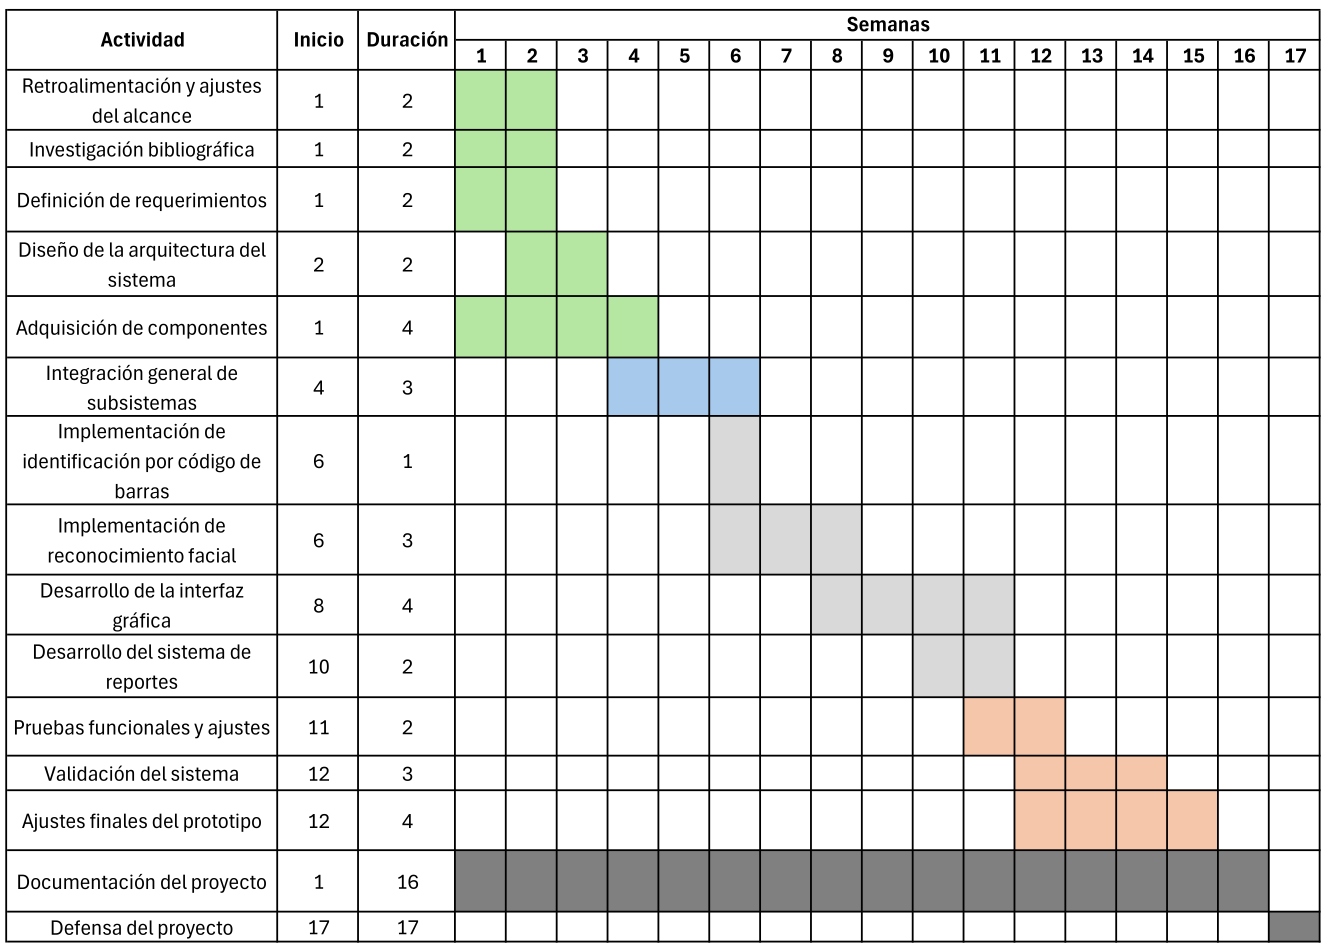
\includegraphics[width=0.6\textwidth]{Figures/SP_21.png}
    \caption{Cronograma propuesto, fuente: elaboración propia}
    \label{fig:ambar}
\end{figure}

\end{frame}

% ============================================================
% Closing slide
% ============================================================

\begin{frame}[plain]

    \centering
    
    \vspace{1.2cm}
    
    {\Huge \textbf{¡Muchas gracias!}}\\[0.4cm]
    
    {\Large por su atención}\\[0.8cm]
    
    \rule{0.75\textwidth}{0.4pt}\\[0.6cm]
    
    {\large \textbf{Diseño y implementación de un sistema de \\ bajo costo para el control ESD en laboratorios de electrónica}}\\[0.2cm]
    {\normalsize Randy Zamora Rojas}\\[0.2cm]
    {\normalsize Asesor: M.Sc Javier Rivera Alvarado}\\[0.8cm]
    
\end{frame}

% ============================================================
% References
% ============================================================

\appendix

\setrightfooter{Referencias}

\begin{frame}[allowframebreaks]{Referencias}

    \tiny
    \bibliographystyle{IEEEtran}
    \bibliography{references}

\end{frame}

% ============================================================
% End document
% ============================================================

\end{document}
